%% Requires compilation with XeLaTeX or LuaLaTeX
\documentclass[10pt,xcolor={table,dvipsnames},t]{beamer}
\usetheme{UCBerkeley}

\title[Your Short Title]{Control Systems}
\subtitle{ }
\author{T.sai varsha\\EE18BTECH11042\\GATE 2017 SET-1 Q.NO 41 (EE SECTION)}
%\institute{Electrical}
%\date{Date of Presentation:15 Feb 2019}

\begin{document}

\begin{frame}
  \titlepage
\end{frame}

% Uncomment these lines for an automatically generated outline.
%\begin{frame}{Outline}
%  \tableofcontents
%\end{frame}

\section{Introduction}

\begin{frame}{Frequency Response}

\begin{itemize}
 For a system having transfer function 
 \begin{equation}
            G(s)= \frac{-s+1}{s+1} ,
 \end{equation} 
 a unit step is applied at time 
 t = 0.
 \begin{itemsize}
 The value of the response of the system at t= 1.5sec is:
  \end{itemsize}
  

\end{itemize}

\begin{block}{}
.
\end{block}

\end{frame}

\section{Some \LaTeX{} Examples}

\subsection{Mathematics}

\begin{frame}{Solution}
We know that, 
\begin{equation}
     x(t) = u(t) 
\end{equation}
 Where u(t) is a unit step input.
 The Laplace transform x(t) is:
 \begin{equation}
     X(s) =  \int_{-\infty}^{\infty}x(t) e^{-st} dt
 \end{equation}
 From this,
 \begin{equation}
     X(s) =  \frac{1}{s}
 \end{equation}
\end{frame}


\subsection{Tables and Figures}

\smallframetitle

\begin{frame}{Solution }

\begin{itemize}
We know that, 
\begin{equation}
  Y(s) = X(s)H(s)
\end{equation}
in Laplace domain.So,
\begin{equation}
Y(s) = \frac{-s+1}{s(s+1)}
\end{equation}
By doing partial fractions,
\begin{equation}
    \frac{-s+1}{s(s+1)} = \frac{A}{s} + \frac{B}{s+1}
\end{equation}


\item  \texttt{} 
\item
\item  \texttt{} 
\end{itemize}


\end{frame}





\begin{frame}
\frametitle{}
By this,
\begin{equation}
A = 1 , B = -2
\end{equation}
From this,
\begin{equation}
    Y(s) = \frac{1}{s} + \frac{-2}{s+1}
\end{equation}
Thw inverse Laplace transform of Y(s) is:
\begin{equation}
    y(t) = u(t) - 2e^{t}u(t)
\end{equation}
u(t) = 1 for all t >0 .So,at t = 1.5sec,
\begin{equation}
    y(1.5) = 1 - 2e^{1}
\end{equation}
\begin{equation}
    y(1.5) = 0.5537
\end{equation}

The value of the response of the system at t = 1.5sec is 0.5537


\end{frame}

\normalframetitle

\begin{frame}
   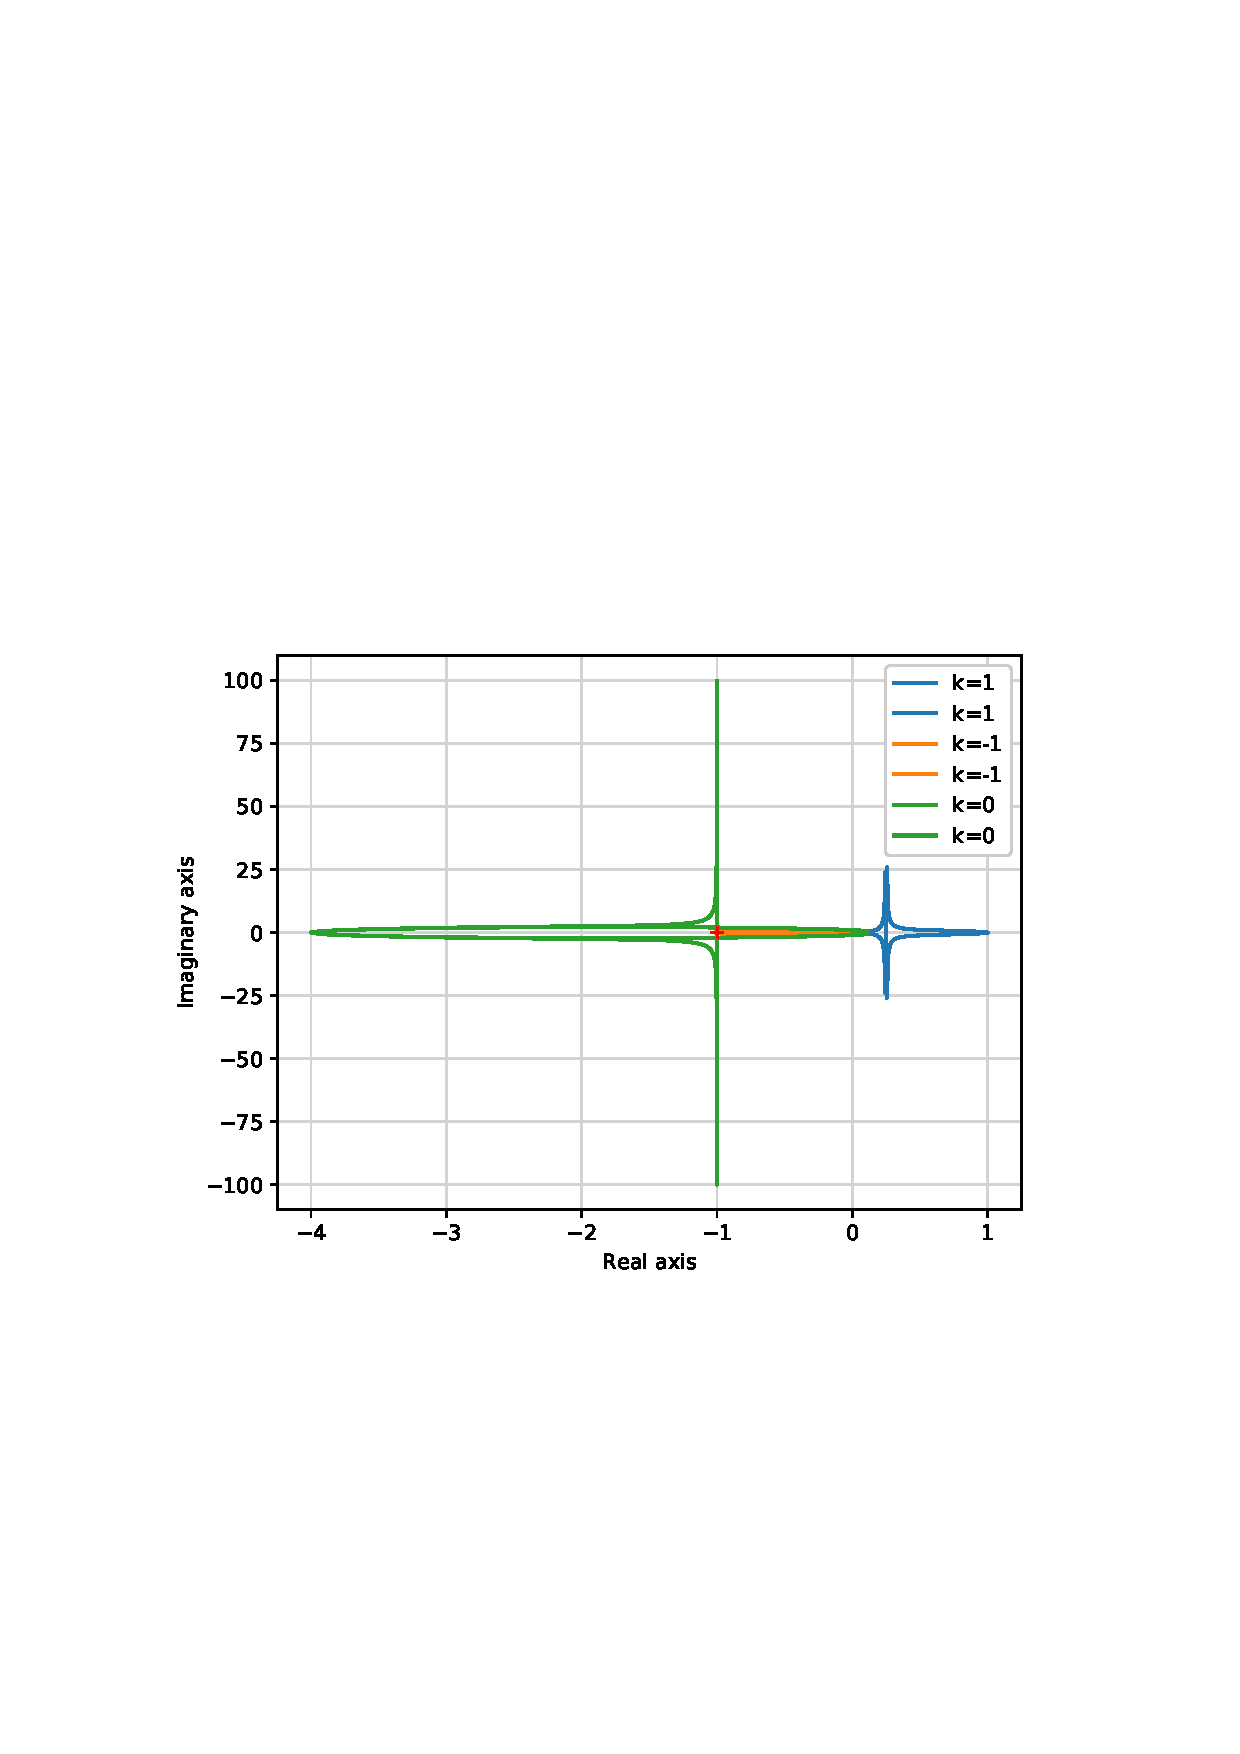
\includegraphics[scale = 0.7]{Figure_1.png}
    
\end{frame}